\subsubsection*{Partie A}

On considère la fonction $f$ définie sur $\mathbb{R}$ par \mbox{$f(x)=\bigl(\dfrac12 x + 1\bigr) \e^{-x}$}.

On note \mbox{$(\mathcal{C}_f)$} sa courbe représentative dans un repère orthonormé.

On admet que la fonction $f$ est dérivable sur $\mathbb{R}$ et on désigne par $f'$ sa fonction dérivée.

\begin{enumerate}
	\item Démontrer que, pour tout réel $x$, \mbox{$f'(x)=\left(-\dfrac12 x -\dfrac12\right) \e^{-x}$}


					\textcolor{red}{\textsc{Correction}}\\
	On utilise la formule \mbox{$\Bigl(u~v\Bigr)~'=u~'~v+v~'~u$,} avec \mbox{$u(x)=\dfrac12 x +1$} donc \mbox{$u~'(x)=\dfrac12$} et \mbox{$v(x)=\e^{-x}$} donc \mbox{$v~'(x)=-\e^{-x}$}.

	Donc \mbox{$f'(x)=\dfrac12 \times \e^{-x}+(\dfrac12x+1)\times(-\e^{-x})=\bigl(\dfrac12-\dfrac12 x-1\bigr) \e^{-x}=\bigl(-\dfrac12 x -\dfrac12\bigr) \e^{-x}$}

	\item Étudier les variations de la fonction $f$ sur $\mathbb{R}$.

						\textcolor{red}{\textsc{Correction}}\\
	L'exponentielle est toujours positive, donc le signe de la dérivée $f'$ ne dépend que du signe de \mbox{$-\dfrac12 x -\dfrac12$}.

	$f'$ est donc positive entre $-\infty$ et $-1$, puis négative.

	On calcule l'image de $-1$ qui est \quad \mbox{$\dfrac12 \e\approx \np{1.35}$}

		\begin{center}
			\begin{tikzpicture}[xscale=1,yscale=1,rotate=0,every node/.style={scale=1,rotate=0}]
			\tkzTabInit[]
			{$x$/0.85,$f~'(x)$/.85,$f(x)$/2.5}
			
			{$-\infty$,$-1$,$+\infty$}
			\tkzTabLine{,+,0,-, }
			\tkzTabVar{-/,+/$\dfrac{\e}{2}$,-/}
		\end{tikzpicture}
		\end{center}

	\item L'affirmation \og{}Pour tout réel $x$, \mbox{$f(x)\leqslant2$}\fg{} est-elle vraie ou fausse ? Justifier.

	\textcolor{red}{\textsc{Correction}}\\
	$f$ atteint en $-1$ son maximum qui est $\dfrac{\e}{2}\approx\np{1.35}$.

	Donc \mbox{$\forall x\in\R, f(x)\leqslant2$}, l'affirmation est vraie.
	\item Déterminer l'équation réduite de la tangente à \mbox{$(\mathcal{C}_f)$} au point d'abscisse 0.

	\textcolor{red}{\textsc{Correction}}\\
	En $0$, on a $f(0)=1$ (c'est l'ordonnée à l'origine) et $f'(0)=-\dfrac12$ (c'est la pente de la tangente).

	Donc l'équation réduite de la tangente en $0$ est \mbox{$y=-\dfrac x 2 +1$}
\end{enumerate}

\subsubsection*{Partie B}

Soit $g$ la fonction polynôme du second degré définie par \mbox{$g(x)=\np{0.5}x^2+bx+c$} où $b$ et $c$ sont deux réels.

On crée la courbe représentée ci-dessous, constituée des deux éléments suivants :
\begin{itemize}[label=$\bullet$]
	\item Une partie de la courbe \mbox{$(\mathcal{C}_f)$} représentative de la fonction $f$ définie dans la partie A sur l'intervalle \mbox{$[-2;0]$}.



	\item Une partie de la courbe \mbox{$(\mathcal{C}_g)$} représentative de la fonction $g$  sur l'intervalle \mbox{$[0;3]$}.
\end{itemize}

\begin{center}
		\begin{tikzpicture}[xscale=1.3,yscale=1.3,rotate=0,every node/.style={scale=1.3,rotate=0}]
	\clip(-3.2,-0.6)rectangle(3.9,4.3);

	\draw[blue!30,thick](-3.2,-0.6)grid(3.9,4.3);
	\draw[blue, line width=0.3mm,->, >=triangle 45](-3.2,0)--(3.9,0);
	\draw[blue, line width=0.3mm,->, >=triangle 45](0,-0.6)--(0,4.3);
	\foreach \i in {-3,-2,-1,1,2,3,4}{\draw(\i,-0.2)node{\textbf{\i}}(-0.2,\i)node{\textbf{\i}};}
	\draw(-0.2,-0.2)node{\textbf{0}};
	\draw[red](-1.5,1.5)node{\mbox{$(\mathcal{C}_f)$}};
	\draw[purple](2.6,2.2)node{\mbox{$(\mathcal{C}_g)$}};
	\draw(0,1)node{x}node[above right]{M};
	\draw[red, line width=0.3mm]plot[smooth,domain=-2:0]	(\x,{(\x/2+1)*exp(-\x)});
	\draw[purple, line width=0.3mm]plot[smooth,domain=0:3](\x,{\x*\x/2-\x/2+1});
\end{tikzpicture}

\end{center}
\vspace{5mm}
Le but de cette partie est de déterminer les valeurs des réels $b$ et $c$.
\begin{enumerate}
	\item Le point \mbox{M~$(0;1)$} appartient aux deux courbes  \mbox{$(\mathcal{C}_f)$} et  \mbox{$(\mathcal{C}_g)$}.

	Démontrer que \mbox{$c=1$}.

		\textcolor{red}{\textsc{Correction}}\\
		\mbox{$g(0)=\np{0.5}\times0^2+b\times0+c=c$}, donc puisque \mbox{$g(0)=1$}, $c=1$.
	\item
 Au point  \mbox{M~$(0;1)$} les courbes  \mbox{$(\mathcal{C}_f)$} et  \mbox{$(\mathcal{C}_g)$} admettent la même tangente.

 Déterminer la valeur de $b$.

 La dérivée de $g$ est \mbox{$g'(x)=x+b$}.

 Donc le nombre dérivé en $0$ est $b$.

 Puisque $f$ et $g$ ont même tangente, on a \mbox{$g'(0)=f'(0)=-\dfrac12$}, donc \mbox{$b=-\dfrac12$.}
\end{enumerate}
